%===========================================================================
%	II. Theoretical Backgrounds
%===========================================================================

The discipline of testing can be found throughout the entire scope of DataOps \cite[42]{Schmidt2019}. However, it does not provide specific testing measures or frameworks. This is because data analytics solutions are tailor-made based on the specific needs of their areas of application. Moreover, available DataOps testing foundations remain a set of guidelines and abstract requirements that need to be applied and customized individually within each DataOps solution.

In this chapter, general DataOps and testing foundations are deduced in order to understand the need for DataOps testing and aid the design process of a use-case-specific testing framework which is to follow in Chapter \ref{chap:testing-framework}.


\section{Introduction to DataOps}
In order to understand the requirement of testing within DataOps, it is important to understand the principles and processes of DataOps itself. In general, DataOps is an approach within building and conducting data analytics which combines established methodologies originating from DevOps, \ac{spc} as well as \textit{agile} software development \cite[24]{Bergh2019}. Several components from each of these methodologies are taken and applied to building and conducting data analytics. These processes aim to eliminate analytics issues found in the traditional development process of such solutions. These issues include but are not limited to slow development and adaptation of analytics solutions \cite{Lockner2019}, error-prone analytics results, repetitive manual processes \cite[11\psqq]{Bergh2019}, etc. Testing is a common component that supports these DataOps processes.

During the rise of DataOps, other terms, including \textit{\acs{ml}Ops}, \textit{\acs{ai}}Ops}, etc., emerged. It is to mention that all data-related \textit{Ops} underlie the general DataOps methodology and focus on specific subsets of data analytics applications.

\subsection{\acs{spc} Heritage: Data Analytics Pipeline}
Common data analytics solutions work by means of a pipeline: Data is acquired from various sources and flows through various steps of transformation, conversion, sanitization, and analysis before resulting in a valuable outcome, e.g., an analytics report. This can be compared to a manufacturing production line. For instance, raw materials from several input points are navigated through a number of steps, resulting in the output product. Issues that might occur during the production flow need to be recognized immediately. It does not suffice to notice issues at the end of a manufacturing process. This is why \acf{spc} is applied to the entire production line. It verifies that each step is conducted correctly and identifies deviations to expected, pre-defined values \cite[1]{Knoth2002}. Applicable tools can then perform recovery measures or stop the process entirely.

This methodology can be directly applied to data analytics pipelines \cite[27]{Bergh2019}. Each step should check if its input, processing, and output is valid and does not carry issues that might lead to unforeseeable problems during further analysis \cite{DataKitchen2020a}. This could help solving the problem of incorrect analytics results since reverse-engineering the origin of the problem is often harder than performing individual checks and fallout measures \cite{Redman2020}. These checks and measures are part of DataOps testing.

\subsection{DevOps Heritage: \acs{cicd} Pipeline Duality, \acs{vcs} and Environment Management} \label{sec:2-1-devops}
DataOps' namesake, DevOps, originates in software development and aims to eliminate manual repetitive processes by automating them. It introduced \acf{cicd} pipelines that take over processes taking place between solution development and deployment. This results in automatic building, testing, and deploying of software solutions \cite[21\psqq]{Kaiser}. This does not only remove repetitive processes but also eliminates so-called \textit{siloed organizations} (i.e., dedicated engineers, testers, operation teams, etc.) depending on each other during a development iteration \cite[56]{Bergh2019}.

In DataOps, enabling \ac{cicd} creates a pipeline duality. This duality is visualized in Figure \ref{fig:2-pipeline-duality}.

\newpage

\begin{figure}[h!]
	\centering
	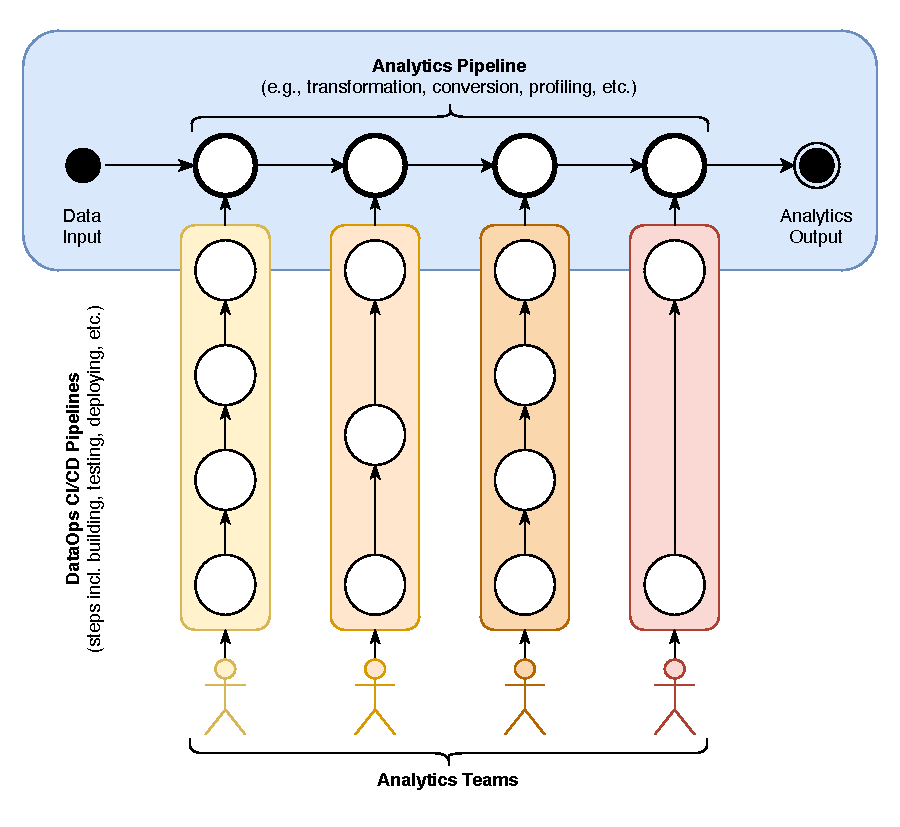
\includegraphics[width=\linewidth]{main-matter/img/2-1-2-pipeline-duality.pdf}
	\caption[DataOps Pipeline Duality]{DataOps Pipeline Duality (per \cite[38\psqq]{Bergh2019})}
	\label{fig:2-pipeline-duality}
\end{figure}

The data analytics (or data operations) pipeline is also called \textit{Value Pipeline} since it is in charge of answering questions through analytical insights \cite[32\psq]{Bergh2019}. Its horizontal representation visualizes its continuous flow. On the contrary, the vertical pipelines, also called \textit{Innovation Pipelines} represent the DataOps \ac{cicd} pipelines \cite[66]{Schmidt2019}. Whenever a new feature is developed for any stage of the pipeline, a number of preliminary steps is performed before finally deploying the solution into production \cite[33]{Bergh2019}. As with data analytics in general, the design of such pipelines highly depends on the analytics and quality requirements. In the scenario of Figure \ref{fig:2-pipeline-duality}, the individual stages require different \ac{cicd} steps and might also be worked on by different teams within the superordinate project.

As with DevOps, DataOps \ac{cicd} ties in with the project's \acf{vcs}. This allows for collaboration between developers as well as development environment management \cite{Davis2020}. Usually, a developer uses an individual sandbox to make changes to the common source code. This sandbox is a highly isolated environment which can be used without impacting the development process of other developers. It includes the current common source code as well as processes for installing and running all required dependencies \cite[41]{Bergh2019}. When committing a change to the \ac{vcs}, it triggers the corresponding \ac{cicd} pipeline which performs its checks and reports potential issues. Otherwise, the updated source code becomes the new common source code since the deployment into production has been conducted successfully.

\subsection{Agile Heritage: Fast-Paced, Iterative Development}
One problem within data analytics is that traditionally developed solutions cannot keep up with the demand of changing requirements. The development process is slow such that valuable and time-dependent information cannot be processed on time \cite{Lockner2019}. In software development, agile development mostly replaced traditional waterfall-orientated processes. \textit{Agile} in DataOps context means that development and improvement is iterative and fast-paced. It requires a \ac{mvp} which is continuously improved by means of previously mentioned \ac{spc} and \ac{cicd} processes \cite[19\psq]{Bergh2019}.

\section{Introduction to Testing}
The previous section introduced where testing aspects can be found within DataOps. This section presents the current state of the art for software and data quality testing. Both disciplines will be evaluated and used within the testing framework design process.

\subsection{Why Do We Need Testing?}
In general, software development relies on testing principles to holistically and objectively validate the expected performance of a piece of software. Nowadays, organizations depend on data analytics more than ever \cite{Munawar2011}. \ac{bi} and \ac{dwh} solutions are designed to utilize data for business-required decision making \cite{Souibgui2019}. While these systems are expected to generate value, many companies lose trust in their data analytics because it might be prone to unforeseeable errors \cite{BISurvey.com}. This is because \ac{bi} and \ac{dwh} systems rely on high-quality data in order to provide representative analytics results and business insights \cite{Munawar2011}. Unfortunately, data quality issues of various sorts and manifestations lead to the systems generating false and potentially misleading reports \cite{Munawar2011}\cite{Freudiger2014}\cite{Redman2016}. Testing the solution for its expected performance at various analytics steps might help solve the underlying issues or even exhaust them completely. 

From a pure software perspective, it is desired that the solution does not break or crash during analytics performance for an unforeseeable reason. Applicable software tests could recognize such issues prior to production deployment, reducing or completely removing crucial bugs inside the software \cite[105\psqq]{ORegan2017}.

\\\

As previously mentioned in Section \ref{sec:2-1-devops}, the pipeline duality ensures continuous flow of both production-grade data analytics as well as improvement and enhancement of the solution. Both pipelines require individual testing measures. This is referred to as \enquote{The Duality of [DataOps] Testing.} \cite[40\sqq]{Bergh2019}

\subsection{Value Pipeline: Data Quality Testing}
Since the Value Pipeline is in charge of the business-critical real-time analysis of various data, the solution-in-use must guarantee the recognition and handling of data quality issues prior, during, and after each individual processing step by means of its \ac{spc} capability. In other words, while the underlying analytics software is static, the variance of data is arbitrarily large and needs to be handled properly. In order to define this kind of event handling, unified data quality dimensions are required.

The \ac{dama} in the United Kingdom defined \enquote{The Six Primary Dimensions for Data Quality Assessment} in 2013 \cite[7\psqq]{Askham2013}. They consist of:

\begin{description}
	\item[Completenes] describes the proportion of the stored data against the potential of being \textit{complete} by means of a use-case-specific completeness definition \cite[8]{Askham2013}\cite{Shen2019}.
	\item[Uniqueness] is achieved when each unique data record only exists once inside the entire database at hand \cite[9]{Askham2013}.
	\item[Timeliness] is the degree to which data represents the reality from the required point in time \cite[10]{Askham2013}.
	\item[Validity] describes a data item corresponding to its expected (and therefore, pre-defined) format, schema, syntax, etc. This definition should also include a range of expected or acceptable variation thresholds \cite[11]{Askham2013}. Testing for data schematics is one processes which allows for definitive objective differentiation between good and bad data \cite{Schieferdecker2012}.
	\item[Accuracy] is the degree to which data \textit{correctly} describes the actual object or event existing in the real world \cite[12]{Askham2013}.
	\item[Consistency] describes the absence of difference when comparing multiple representations of the same real-life object against its actual definition \cite[13]{Askham2013}.
\end{description}

It can be seen that the areas of data quality are mostly covered when data complies with the corresponding data governance definitions \cite{Schieferdecker2012}. These definitions build the foundation for a valid testing framework.

In practice, checks based on these dimensions have to be embodied inside the data analytics solution. Based on mentioned, use-case-specific requirements, a data flow can be checked by means of those dimensions, leading to recovery measures inside the system, or a system failure with appropriate error reporting.

\subsection{Innovation Pipelines: Software Testing}
Section \ref{sec:2-1-devops} describes the Innovation Pipelines as DataOps-specific \ac{cicd} pipelines. Apart from the build and deployment process, a major part of these pipelines is represented by software testing. Whenever a developer intends to update the codebase, a number of tests of various levels is conducted, visualized in the pyramid graphic in Figure \ref{fig:2-testing-pyramid} below.

Depending on the type of software, the types and levels of testing can vary. For data analytics solutions with \acp{ui} outside their scope, the three foundational levels suffice.

\begin{figure}[h!]
	\centering
	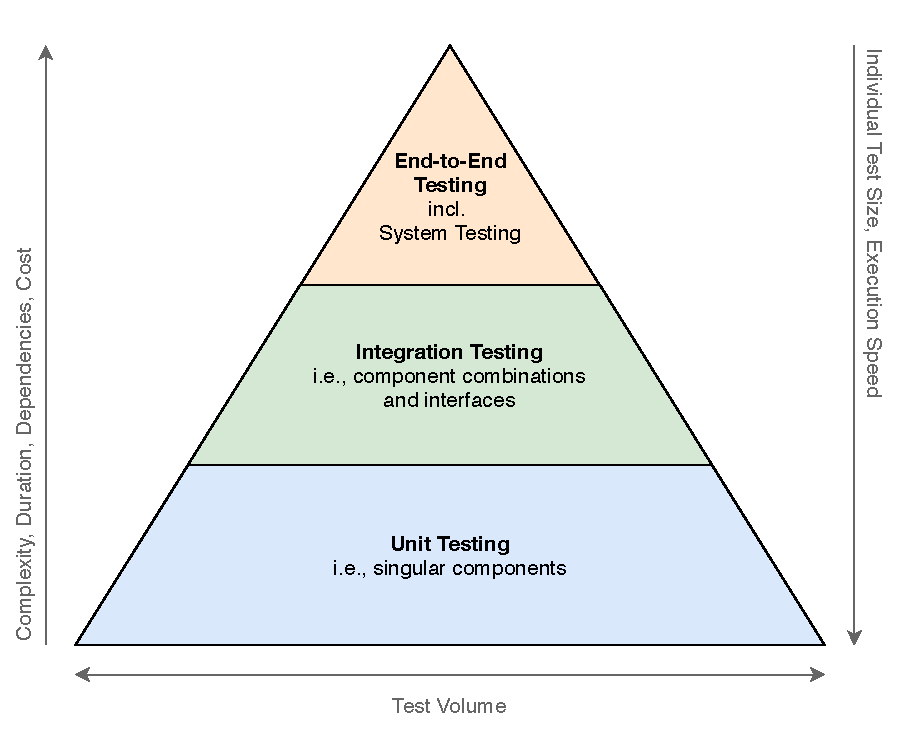
\includegraphics{main-matter/img/2-2-3-testing-pyramid.pdf}
	\caption{Software Testing Level Pyramid}
	\label{fig:2-testing-pyramid}
\end{figure}

\newpage



\begin{description}
	\item[Unit Tests] take individual components (i.e., \textit{units}) from the source code and check their behavior. Unit tests are pieces of code that invoke the chosen test unit and compare its actual result with the expected outcome \cite[sec. 1]{Osherove2013}. They are characterized as granular, thus highly voluminous, repeatable, isolated, and idempotent \cite[sec. 2]{Osherove2013}.
	\item[Integration Test] verify that multiple combined units are working together as expected. They focus on testing of interfaces that connect singular components \cite[66]{Mahfuz2016}. Integration tests are performed in a less isolated environment, resulting in more outside dependencies \cite[sec. 3]{Osherove2013}.
	\item[End-to-End Tests] describe the highest level of software testing \cite[67]{Mahfuz2016}. For the sake of simplicity, system tests are treated as a part of end-to-end tests within this work. End-to-end tests are performed under a (close-to) deployment situation. This creates an idealized real-life scenario. Thus, end-to-end testing is the least isolated level and serves as the final test stage before actual deployment. \cite[67]{Mahfuz2016}.
\end{description}



Those three layers represent the \textit{Fuctional Testing} type since they are built based on the functional requirements of a software solution \cite[69]{Mahfuz2016}. Its counterpart, \textit{Non-Functional Testing}, covers aspects like load, performance, security, etc. \cite[70]{Mahfuz2016}.

Apart from that, other testing methods can be applied to each testing layer. \textit{Smoke Tests} are a subset within the entire test suite that cover core functionality required for the solution to \textit{just} run. Such tests can help to recognize the complexity of a software issue \cite[sec. 5]{Tarlinder2016}. Conducting \textit{Regression Tests} is also important. They aim to uncover errors with pre-existing components when other components were newly included, changed, or removed \cite[70]{Mahfuz2016}\cite{Mathur2013}. This is especially crucial with data analytics solutions since historic data still needs to be processable after updating the analytics engine \cite{Shen2019}. To achieve regression testing in practice, unit tests can be written in a more abstract manner and re-run for the entire software solution, requiring older unit tests still to pass \cite{Mathur2013}.
\\\
Putting everything into DataOps perspective, the Innovation Pipelines need to cover source code changes of the analytics solution. These \ac{cicd} pipelines need to embody traditional software tests to verify the correct behavior of the application. This also includes testing the \ac{spc} capability of the given solution \cite{DataKitchen2020}. For that reason, pathological test data needs to be provided that is able to invoke a majority of realistic events during the analytics process \cite[42]{Bergh2019}. In case of tests failing, the corresponding \ac{cicd} Innovation Pipeline can report the issue back to the developer, allowing for further understanding and correction.

All in all, these tests are expected to invoke the majority of outcome possibilities, leading to a high test coverage and correct performance validation \cite{DataKitchen2020a}.

  










